\chapter{IR using Relational Databases}
\label{ir-using-relational-databases}
\epigraph{``Is this new question a worthy one to investigate?'' This latter question we investigate without further ado, thereby cutting short an infinite regress.}{Alan Turing - 1950}

\begin{Abstract}
	\begin{changemargin}{1cm}{1cm}
		There have been many attempts to express information retrieval problems using relational databases. In this chapter, one of the latter attempts that revived the idea of expressing bag-of-words ranking functions using SQL will be highlighted. A prototype system that uses these expressions is presented, dubbed OldDog. This system can be used for rapid IR prototyping and is especially helpful in the context of reproducible information retrieval research.
		Also, when researchers speak of BM25, it is not always clear which variant they mean since many tweaks to \citeauthor{bm25-robertson}'s original formulation have been proposed. Does this ambiguity ``matter''? We attempt to answer this question with a large-scale reproducibility study of BM25, considering eight variants implemented in the OldDog system. Experiments on three newswire collections show no significant effectiveness differences between them, including Lucene's often maligned approximation of document length.
	\end{changemargin}
\end{Abstract}

\section{Introduction}
Where information retrieval researchers commonly use inverted indexes as data structures, there is also a rich history of researchers using relational databases to represent the data in information retrieval systems. Different approaches in the literature present varying successes. Given this context, we arrive at the first research question: 
\begin{itemize}
	\item[\textbf{RQ1:}] What are the benefits of using relational databases for information retrieval?
\end{itemize}
In order to answer this question, first, we will look at the history of using database systems for IR. Then, one of the latter attempts of using a relational database for information retrieval will be highlighted. Using this work a prototype system is built, dubbed ``OldDog''. This system will be used in a reproduction experiment, which compares several variants of BM25 which each other. This reproduction study does not only confirm previous findings found in the literature, it also verifies that relational databases systems are suited for running IR experiments. 

\section{Related work}

\subsection{Boolean retrieval}
Perhaps the earliest work on using relational databases for information retrieval is the work by~\citet{SchekPistor}. In their work, the authors recognize that the relational data model is widely accepted as an interface to query structured data. However, in cases of unstructured data, like text, it is inconvenient to use. They proposed an extension for the relational model by allowing Non First Normal Form ($\text{NF}^2$) relations. This extension allows for text queries to be more easily expressed. However, the systems that can be built in this language are boolean retrieval systems. Which at the time worked well, but scoring was not a feature implemented.  
Similarly, \citet{macleod} compared the relational model with the inverted index model. \Citeauthor{macleod} showed how queries of the IBM STAIRS system could be expressed using the relational model. These were, however, still boolean queries, so scoring using uncertainty was not considered. 

\subsection{Probabilistic Relational Algebra}
\Citet{fuhr1996probabilistic} recognized that where databases contain formatted data, IR systems deal with unformatted data, which requires uncertain inference. They propose to express this uncertainty using a probabilistic relational algebra~\citep{fuhr-pra} (PRA). 
PRA can be considered an extension of standard relational algebra. 
The basic idea behind PRA is that tuples are assigned weights; the weight represents the probability that the tuple belongs to the relation. These probabilities give two advantages. Uncertain information can be expressed, and tuples representing answers to queries can be ordered by the weights representing the uncertainty. The most certain tuples are ranked at the top. Although these extensions give advantages over boolean retrieval, how to assign these probabilities to, for example, a document-term pair remains a question.

\subsection{IR on top of a database cluster}
% T. Grabs, K. Bhoem, and H.-J. Schek. PowerDB-IR: scalable information retrieval and storage with a cluster of databases. Knowledge and Information Systems, 6(4):465–505, 2004.
\Citet{PowerDB-IR} propose PowerDB-IR, developed to run IR applications on a scalable infrastructure. It should also be able to update the data quickly while retrieving up-to-date results. \Citeauthor{PowerDB-IR} achieve this by assigning every document to a category, e.g., sports or news. In their experiments, they use 16 artificial categories. A dedicated node is created for every category, containing tables containing documents, inverted lists, and statistics tables. 
The system supports both single-category and multi-category searches. For a single query search, the following ranking score value is calculated:
\begin{equation}
	\text{RSV}(d,q) = \sum_{t\in q} \mathit{tf}(t, d) \cdot \mathit{idf}(t)^2 \cdot \mathit{tf}(t, q)
\end{equation}
Here $\mathit{tf}(t, d)$ is the term frequency of term $t$ in document $d$, $\mathit{idf}(t)$ is the inverted document frequency of term $t$ (which is squared in this formula), and $\mathit{tf}(t, q)$ is the term frequency of term $t$ in the query text. Calculating this is straightforward: all statistics necessary are stored on a node. However, when one wants to search on multiple (or all) categories.
The cost of this approach is high, but this work may have proposed the first real IR in SQL approach. 

\subsection{Integrating DB + IR}
% S. Chaudhuri, R. Ramakrishnan, and G. Weikum. Integrating DB and IR technologies: What is the sound of one hand clapping? CIDR, 2005.
\Citet{Chaudhuri2005IntegratingDA} also identify the need for systems that integrate both database and IR functionalities. In their view, database systems need to be more flexible for scoring and ranking, while IR systems can not handle structured data and metadata properly. \Citeauthor{Chaudhuri2005IntegratingDA} put together a list of seven requirements that a DB + IR system should be able to support, of which they identify the following three requirements as the most important:
\begin{enumerate}
	\item \emph{Flexible scoring and ranking.}
	It should be possible to customize the ranking function for different applications; a news search system probably needs different ranking functions and settings than a web search system. 
	\item \emph{Optimizability.}
	Following standard database approaches, queries in a DB+IR system should have a query optimizer that considers the workload and the data characteristics. For example, when only one relevant result is sufficient, the system should be able to abort when a relevant document is found. 
	\item \emph{Metadata and ontologies.}
	Other than metadata that describes data sources, other metadata that is used for understanding information demands might be needed. This metadata could be, for example, an ontology or a lexicon used for more effective ranking strategies.\footnote{Latent representations generated by large language models are a great example of this kind of metadata.}
\end{enumerate}
To build a system that can support these requirements, the authors identify four alternatives for designing a DB+IR system:
\begin{enumerate}
	\item \emph{On-top-of-SQL.} The IR functionalities are built on top of a SQL engine. The disadvantage of this approach is that it is challenging to customize efficient access for both IR and DB functionalities. 
	\item \emph{Middleware.} In this approach, a SQL engine and an IR engine are run simultaneously. The two disadvantages of using this approach are that the API needs to talk to two systems, which can have very different design philosophies, and the data needs to be shared between systems, incurring a large overhead and making it harder to combine both functionalities. 
	\item \emph{IR-via-ADT's.} The third approach is building an IR system using abstract data types. The authors argue that this approach makes the system more customizable than the previous approaches. However, the authors also note that optimization in the case of UDFs is complicated. Also, when programmers need to work with such a system, it has the full complexity of SQL plus the complexity of working with ADTs, making them efficient. 
	\item \emph{RISC.} The final approach is what the authors prefer; IR functionalities build on top of a relational \textit{storage} engine, as described in an earlier work by them~\citep{risc}. The DB+IR systems should then be built on top of this engine. 
\end{enumerate}  
Although the approaches described in this work are interesting, they do not provide prototypes to compare them. (The goal of this paper was to present a theoretical framework for tackling this problem.)

\subsection{Handwritten plans and Array Databases}
% S. H´eman, M. Zukowski, A. de Vries, and P. A. Boncz. MonetDB/X100 at the 2006 TREC terabyte track. TREC, 2006.
\Citet{handwritten} participated in the TREC TeraByte track using the relational engine MonetDB/X100 \citep{monetdb/x100}. They were able to express ranking functions efficiently and effectively in this system. In their submission, they used BM25 as a scoring function. In order to reduce the amount of computing necessary for every document-term pair, the BM25 score was precalculated. 
The disadvantage of this approach was that the query plans were not generated from SQL but were handwritten. Having to handwrite queries makes this system more challenging to use for IR researchers. Also, because all BM25 scores were precalculated (albeit with some compression), more storage was needed than when only the term frequencies were saved.

% R. Cornacchia, S. H´eman, M. Zukowski, A. de Vries, and P. Boncz. Flexible and efficient IR using array databases. VLDB, 2008.
The same research group~\citep{array-db} also ran experiments on the TREC TeraByte track using the array database SRAM (Sparse Relational Array Mapping). SRAM automatically translate BM25 queries to run them on a relational engine (particularly X100). However, SRAM is quite an exotic query language, only used by some researchers. 

\subsection{Retrieval models only using SQL}
In more recent work, \citet{OldDog} showed that the commonly used BM25 ranking function could also be easily expressed using SQL. This is done similarly to \citet{PowerDB-IR}. In this work, the MonetDB~\citep{monet} and Vectorwise~\citep{vectorwise} systems were used, making it much faster. \Citeauthor{OldDog} specifically focused on the retrieval efficiency of several systems. They argue that instead of using a custom build IR system using an inverted index, researchers could store their data representations in a column-oriented relational database and formulate the ranking functions using SQL. They show that their implementation of BM25 in SQL is on par in efficiency and effectiveness compared to systems that use an inverted index.\footnote{In particular the Vectorwise system.}  

There was an interesting observation in the paper to highlight: All the systems evaluated in this paper implement BM25. However, there was a substantial difference between the effectiveness scores produced by these systems, as shown in \cref{olddog_results}. The only two systems that achieved the same effectiveness score were the two database systems (MonetDB and Vectorwise). However, these two systems were developed by the same research group.

\begin{table}[!ht]
	\centering
	\caption{Results presented by \citet{OldDog}. \texttt{MAP} and \texttt{P@5} on the ClueWeb12 collection are reported for five different systems that run BM25. The table shows that only the two database systems (MonetDB and Vectorwise) achieve the same effectiveness score.}
	\label{olddog_results}
	\begin{tabular}{c c c}
		\toprule
		System &  \texttt{MAP} & \texttt{P@5} \\
		\midrule
		Indri~\citep{indri} & 0.246 & 0.304 \\
		MonetDB~\citep{monet} & 0.225 & 0.276 \\
		Vectorwise~\citep{vectorwise} & 0.225 & 0.276 \\
		Lucene~\citep{lucene} & 0.216 & 0.265 \\
		Terrier~\citep{terrier} & 0.215 & 0.272 \\
		\bottomrule
	\end{tabular}
\end{table}

These results were surprising as the authors took specific care to keep document preprocessing identical for all systems. However, the observed difference in \texttt{MAP} of 3\% absolute was the largest deviation in the score reported.

\subsection{Reproducibility}
Not only did we observe the differences in effectiveness scores for BM25 in the paper by \citet{OldDog}. In the SIGIR 2015 Workshop on Reproducibility, Inexplicability, and Generalizability of Results (RIGOR)~\citep{RIGOR} and the Open-Source IR Replicability Challenge (OSIRRC) workshop~\citep{OSIRRC} similar results are observed. See \cref{rigor_results} and \cref{osirrc_results} respectively.  

\begin{table}
	\centering
	\caption{Results from the RIGOR workshop~\citep{RIGOR}. \texttt{MAP@1000} on the .GOV2 collection is reported for four different systems that run BM25. The table shows that all four implementations report a different effectiveness score.}
	\label{rigor_results}
	\begin{tabular}{c c}
		\toprule
		System &  \texttt{MAP@1000} \\
		\midrule
		ATIRE~\citep{ATIRE} & 0.290 \\
		Lucene~\citep{lucene} & 0.303 \\
		MG4J~\citep{MG4J} & 0.299 \\
		Terrier~\citep{terrier} & 0.270 \\
		\bottomrule
	\end{tabular}
\end{table}

\begin{table}
	\centering
	\caption{Results from the OSIRRC workshop~\citep{OSIRRC}. \texttt{AP}, \texttt{P@30}, and \texttt{NDCG@20} on the robust04 collection are reported for seven different systems that run BM25. As shown in the table, all implementations report (again) a different effectiveness score.}
	\label{osirrc_results}
	\begin{tabular}{c c c c}
		\toprule
		System & \texttt{AP} & \texttt{P@30} & \texttt{NDCG@20} \\
		\midrule
		Anserini~\citep{anserini-docker} & 0.253 & 0.310 & 0.424 \\
		ATIRE~\citep{ATIRE} & 0.218 & 0.320 & 0.421 \\
		ielab~\citep{ielab} & 0.183 & 0.261 & 0.348 \\
		Indri~\citep{indri-docker} & 0.239 & 0.300 & 0.404 \\
		OldDog~\citep{olddog-docker} & 0.243 & 0.299 & 0.400 \\
		Pisa~\cite{pisa} & 0.253 & 0.312 & 0.422 \\
		Terrier~\citep{terrier-docker} & 0.236 & 0.298 & 0.405 \\
		\bottomrule
	\end{tabular}
\end{table}

It is unclear why the results between these systems differ this much; many explanations are possible. Examples include; different preprocessing\footnote{But not in~\citeauthor{OldDog}, as they ensured preprocessing was the same for all systems.}, different hyperparameter settings, other functions for inverse document frequency ($idf$), or erroneous implementation of the ranking function. Using, for example, non-optimized hyperparameter settings can lead to considerable gaps in differences between effectiveness scores. \citet{weak-baselines} showed that in many cases, new ranking methods had been proposed that compared the results of a newly proposed method to a non-fine-tuned version of BM25, making the results look better than they are. The choices for hyperparameters are often left out of papers, while BM25 is the baseline compared against. As BM25 is often used as a baseline, it is important to understand why these difference exists, and how they arise.

\section{Prototype OldDog}
As shown in \cref{osirrc_results}, one of the submissions to the workshop was by us~\citep{olddog-docker}. This prototype is a software project to replicate and extend the database approach to information retrieval presented in \citet{OldDog}. As the prototype was based on their work, we dub it \emph{OldDog}. OldDog uses column store database MonetDB~\citep{monet} for query processing. 
\Citeauthor{OldDog} produced the database tables to represent ``postings'' using a custom program running on Hadoop.
Instead, we relied on the Anserini toolsuite~\cite{anserini} to create a
Lucene index. From this index, we extracted the data necessary to fill the tables. Anserini takes care of standard document preprocessing. The ranking function implemented in OldDog was BM25 as proposed by \citet{bm25-robertson}.

\subsection{Docker}
For the submission to the OSIRRC workshop~\citep{OSIRRC}, we created a docker image of OldDog\footnote{\url{https://hub.docker.com/r/osirrc2019/olddog}}. \Citeauthor{OldDog} implemented a conjunctive variant of BM25 (all query terms have to be present in a document in order for a document to be considered relevant). When creating the submission for the workshop, we noticed that the effectiveness scores were substantially lower than other submissions. When removing the conjunctive constraint, the effectiveness results increased. So our prototype supports both conjunctive and disjunctive versions of BM25. Our entry in \cref{osirrc_results} presents the effectiveness scores of the disjunctive variant. The retrieval effectiveness degraded more than we expected a priori, given the results in previous work. The number of relevant documents per topic for this collection was likely relatively low.

\subsection{Ease-of-Use}
Having implemented BM25 in a database system enabled us to carry out some experiments quite easily that are more mundane when using an inverted index. As all document frequencies are stored in one table, filtering out the terms with a large document frequency is easy. In only two lines of SQL, we updated the table removing the terms with large document frequency, as shown in \cref{fig:remove-high-df}. This approach could be an automatic way to remove stopwords from a collection. This filter was too strict to improve retrieval effectiveness but can easily be fine-tuned.

\begin{figure}
	\begin{minted}[linenos, breaklines, breakafter=-, escapeinside=||]{sql}
ALTER TABLE dict 
RENAME TO odict;
CREATE table dict 
AS SELECT * FROM odict WHERE df <= (
	SELECT 0.1 * COUNT(*) FROM docs
);		
	\end{minted}
	\caption{This code updates the \texttt{docs} table such that all terms with a document frequency greater than a tenth of the collection size are removed.}
	\label{fig:remove-high-df}
\end{figure}

\section{Variants of BM25}
Having ``OldDog'' set up, we can quickly run retrieval experiments. As mentioned in the previous section, it is still unclear why the differences between the submissions were this big. Also, many different variants of BM25 that claim to be more effective have been proposed in the literature. A study by \citet{trotman-bm25} compared several variants and found that improvements presented in the literature do not add up. 
As we now have a system in which the BM25 formula is written directly in SQL, we can easily swap this version of BM25 with its proposed improvements. By using OldDog, we can ensure the data representation is the same when we compare these variants; the results will only reflect what the effects are applying a different variant of BM25. This way, we can easily confirm the findings of \citeauthor{trotman-bm25}.

\subsubsection{\Citet{bm25-robertson}} 
The original formulation of BM25 is constructed from two parts. The first part is derived from the binary independence relevance model~\citep{bm25-beyond}, which results in an approximation of the classical inverse document frequency ($\mathit{idf}$) for a query term $t$:

\begin{equation} 
	w_i^{\text{IDF}} = \log\left(\frac{N-\mathit{df}_t+0.5}{\mathit{df}_t+0.5}\right)
\end{equation}
where $N$ is the collection size, and $df_t$ are the number of documents in the collection that contain query term $t$.  

There is, however, a negative consequence of using this formula for weighing term importance. Let us say there is a collection with $10,000$ documents; then, it is possible to plot the $\mathit{idf}$ for each term as shown in~\cref{idf}. The figure shows that the $\mathit{idf}$ score becomes negative when $\mathit{df}_t > \frac{N}{2}$. This happens for terms that appear in more than half of all documents, e.g.: ``the'' or ``a''. Many systems do not consider these terms when searching by keeping a list of common words that can be ignored (stop words). However, when these words are considered,  a negative $\mathit{idf}$ would decrease the relevance scores of documents with the query term in the document—some variations of BM25 deal with this, which are discussed in the following sections.  

\begin{figure}
	\caption{Inverse document frequency as used by \citet{bm25-robertson}}
	\label{idf}
	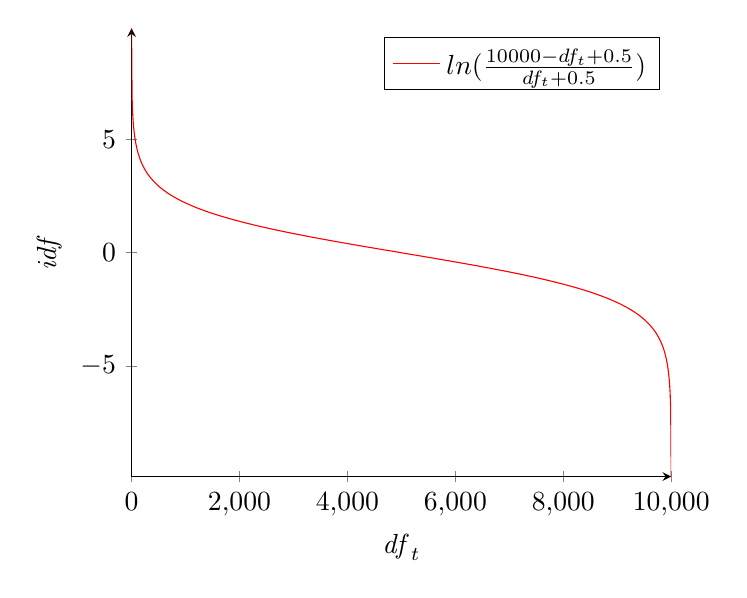
\begin{tikzpicture}
		\begin{axis}[
			axis lines = left,
			xlabel = \(\mathit{df}_t\),
			ylabel = {\(\mathit{idf}\)},
			]
			%Below the red parabola is defined
			\addplot [
			domain=0:10000, 
			samples=1000, 
			color=red,
			]
			{ln((10000-x+0.5)/(x+0.5))};
			\addlegendentry{\(ln(\frac{10000-df_t+0.5}{df_t+0.5})\)}
		\end{axis}
	\end{tikzpicture}
\end{figure}

The second part of BM25 can be considered as a term frequency weighting $\mathit{tf}$. These two parts are multiplied to get something like the traditional term frequency-inverse document frequency weighting $\mathit{tf} \times w_i^{\text{IDF}}$.
However, the $\mathit{tf}$ in BM25 is extended: every additional term occurrence does not increase the ranking score value as much as the previous one. For example, a term being present twice in a document versus once provides more information than a term being present ten times versus nine. For this, the following convenient formula as a replacement for \textit{tf} was chosen:

\begin{align}
	\frac{\mathit{tf}}{k+\mathit{tf}} & \text{ where } k>0
\end{align}

This approach ensures that the term frequency does not increase linearly. In the final formulation of BM25, $k$ is written as $k_1$. This is because earlier versions of this ranking formula also had a $k_2$ and $k_3$ parameter. 

Then lastly, a second component is added that can correct for documents longer than others. It is, however, not clear how one should deal with documents being longer than others; the author of a document can be verbose, in which case additional term occurrences do not provide any more information. On the other hand, a lengthy document can be because more relevant information is provided, and the document is more relevant than its shorter counterpart. For these reasons, the following soft-length normalization is introduced:

\begin{align}
	\left(1-b\right) + b \times \left(\frac{L_d}{L_{\mathit{avg}}}\right) & \text{ with } 0 <= b <= 1
\end{align}

When setting $b=1$, full-length normalization is used, while if $b=0$, none is used. Combining these parts, including the correction for term frequency and the length normalization, we get BM25 as initially proposed by \citet{bm25-robertson}:

\begin{equation}
	\label{bm25-robertson}
	\sum_{t\in q} \log\left(\frac{N-\mathit{df}_t+0.5}{df_t+0.5}\right)\cdot\frac{\mathit{tf}_{\mathit{td}}}{k_1\cdot\left(1-b+b\cdot\left(\frac{L_d}{L_{\mathit{avg}}}\right)\right) + \mathit{tf}_{\mathit{td}}}
\end{equation}

\subsubsection{Lucene (default)}
The variant implemented in Lucene (as of version 8) introduces two main differences. First, since the $\mathit{idf}$ component of \citet{bm25-robertson} is negative when:

\begin{equation}
	\mathit{df}_t > \frac{N}{2} 
\end{equation}

To avoid negative values in all possible cases, Lucene adds a constant one before calculating the $log$ value. 
Second, the document length used in the scoring function is compressed (in a lossy manner) to a one-byte value, denoted $L_{d\text{lossy}}$. With only 256 distinct document lengths, Lucene can pre-compute the value of

\begin{equation}
	k_1 \cdot \left(1-b+b\cdot\left(\frac{L_{d\text{lossy}}}{L_{\mathit{avg}}}\right)\right)
\end{equation}

for each possible length, resulting in fewer computations at query time. Then \cref{lucene-default} describes BM25 as implemented in Lucene:

\begin{equation}
	\label{lucene-default}
	\sum_{t\in q}\log\left(1 + \frac{N-\mathit{df}_t+0.5}{\mathit{df}_t+0.5}\right)\cdot\frac{\mathit{tf}_{\mathit{td}}}{k_1\cdot\left(1-b+b\cdot\left(\frac{L_{d \text{lossy}}}{L_{\mathit{avg}}}\right)\right)+\mathit{tf}_{\mathit{td}}}
\end{equation}

\subsubsection{Lucene (accurate)}

\Cref{lucene-accurate} represents our attempt to measure the impact of Lucene’s lossy document length encoding. We implemented a variant that uses exact document lengths but is otherwise identical to the Lucene default.

\begin{equation}
	\label{lucene-accurate}
	\sum_{t\in q}\log\left(1 + \frac{N-\mathit{df}_t+0.5}{\mathit{df}_t+0.5}\right)\cdot\frac{\mathit{tf}_{\mathit{td}}}{k_1\cdot \left(1-b+b\cdot\left(\frac{L_d}{L_{\mathit{avg}}}\right)\right)+\mathit{tf}_{\mathit{td}}}
\end{equation}

\subsubsection{ATIRE~\citep{ATIRE}}
\Cref{atire-variant} shows BM25 as implemented by ATIRE; it implements the $\mathit{idf}$ component of BM25 as $\log(N/\mathit{df}_{t})$, which also avoids negative values. The TF component is multiplied by $k_1+1$ to make it look more like the classic RSJ weight~\citep{RSJ}; this does not affect the resulting ranked list, as all scores are scaled linearly with this factor.

\begin{equation}
	\label{atire-variant}
	\sum_{t\in q}\log\left(\frac{N}{\mathit{df}_t}\right)\cdot\frac{\left(k_1 + 1\right)\cdot \mathit{tf}_{\mathit{td}}}{k_1\cdot\left(1-b+b\cdot\left(\frac{L_{d}}{L_{\mathit{avg}}}\right)\right)+\mathit{tf}_{\mathit{td}}}
\end{equation}

\subsubsection{BM25L~\citep{bm25l}}
BM25L builds on the observation that BM25 penalizes longer documents too much compared to shorter ones. The $\mathit{idf}$ component differs to avoid negative values. The TF component is reformulated as follows:
\begin{equation}
	\frac{\left(k_1+1\right)\cdot c_{\mathit{td}}}{k_1+c_{\mathit{td}}}  
\end{equation}
with 

\begin{equation}
	c_{\mathit{td}} = \frac{\mathit{tf}_{\mathit{td}}}{1 - b + b \cdot \left(\frac{L_d}{L_{\mathit{avg}}}\right)}  
\end{equation}
The $c_{td}$ component is further modified by adding a constant $\delta$, boosting the score for longer documents. The authors report using $\delta = 0.5$ for the highest effectiveness. \Cref{bm25l} presents the final formulation of BM25L:

\begin{equation}
	\label{bm25l}
	\sum_{t\in q} \log\left(\frac{N+1}{\mathit{df}_t + 0.5}\right)\cdot\frac{(k_1 + 1)\cdot(c_{\mathit{td}} + \delta)}{k_1 + (c_{\mathit{td}} + \delta)}
\end{equation}

\subsubsection{BM25+~\citep{bm25+}}
BM25+, as shown in \cref{bm25+}, encodes a general approach for dealing with the issue that ranking functions unfairly prefer shorter documents over longer ones. \Citeauthor{bm25+} propose adding a lower-bound bonus when a term appears at least once in a document. The difference with BM25L is a constant $\delta$ to the TF component. The $\mathit{idf}$ component is again changed to a variant that disallows negative values.

\begin{equation}
	\label{bm25+}
	\sum_{t\in q} \log\left(\frac{N+1}{\mathit{df}_t}\right)\cdot\left(\frac{\left(k_1 + 1\right)\cdot \mathit{tf}_{\mathit{td}}}{k_1\cdot\left(\left(1-b\right)+b\cdot\left(\frac{L_d}{L_{\mathit{avg}}}\right)\right)+\mathit{tf}_{\mathit{td}}}+\delta\right)
\end{equation}

\subsubsection{BM25-adpt~\citep{bm25-adpt}}
BM25-adpt is an approach that varies $k_1$ per term (i.e., uses term specific $k_1$ values). In the original formulation of BM25, $k_1$ can be considered a hyperparameter that regulates the increase of score for additional occurrences of a term; $k_1$ ensures that every additional occurrence gets discounted as it provides less information than its previous. However, \citeauthor{bm25-adpt} argued that this does not necessarily have to be the case. If there are fewer documents with $t+1$ occurrences versus $t$, it should provide more information compared to when the number of documents is almost the same. In order to find the optimal term-specific $k_1$ value, the authors want to maximize the information gain for that particular query term. 
First, they identify the probability of selecting a document randomly from the collection that contains the term $q$ at least once in a document as:

\begin{equation}
	p(1|0,q) = \frac{\mathit{df}_t+0.5}{N+1}
\end{equation}

The probability of a term occurring one more time is defined as:

\begin{equation}
	p(t+1|t,q) = \frac{\mathit{df}_{t+1}+0.5}{\mathit{df}_t+1}
\end{equation}

In both these formulas, $1$ and $0.5$ are added for smoothing to avoid zero probabilities. Then the information gain from $t$ to $t+1$ occurrences is computed as, subtracting the initial probability: 

\begin{equation}
	G^t_q = \log_2\left(\frac{\mathit{df}_{t+1} + 0.5}{\mathit{df}_t+1}\right) - \log_2 \left(\frac{\mathit{df}_{t} + 0.5}{N+1}\right)
\end{equation}

Here $\mathit{df}_t$ is not defined as a standard document frequency but based on the length normalized term frequency:

\begin{equation}
	df_t = 
	\begin{cases}
		|D_{t|c_{td}\geq t-0.5}| & t > 1\\ 
		df(q) & t = 1\\
		N & t = 0
	\end{cases}
\end{equation}

In this case $\mathit{df}(q)$ is the ``normal'' document frequency, and $c_{\mathit{td}}$ is the same as in BM25L (pivoted method for length normalization~\cite{ctd}):

\begin{equation}
	c_{\mathit{td}} = \frac{\mathit{tf}_{\mathit{td}}}{1-b+b\cdot\left(\frac{L_d}{L_{\mathit{avg}}}\right)}
\end{equation}

This means the following: $\mathit{df}_t$ is equal to the number of documents in the collection when $t = 0$, and it is equal to the ``normal'' document frequency when $t = 1$. Otherwise, it will be the number of documents with at least $t$ occurrences of the term (rounded up) using the pivoted method $c_{\mathit{td}}$. 

Then, the information gain is calculated for $t \in \{0,\cdots,T\}$,until $G^t_q > G^{t+1}_q$. This threshold is chosen as a heuristic: When $t$ becomes large, the estimated information gain can be very noisy. So $T$ is chosen as the smallest value that breaks the worst burstiness rule~\citep{burstiness_rule} (the information gain starts decreasing). The optimal value for $k_1$ is then determined by finding the value for $k_1$ that minimizes the following equation:
\begin{equation}
	k'_1 = \argmin_{k_1} \sum_{t=0}^{T}\left(\frac{G^t_q}{G^1_q} - \frac{(k_1+1)\cdot t}{k_1+t}\right)^2
\end{equation}

Essentially, this gives a value for $k_1$ that maximizes information gain for that specific term; $k_1$ and $G^1_q$ are then plugged into the BM25-adpt formula: 

\begin{equation}
	\label{bm25-adpt}
	\sum_{t\in q}G_q^1\cdot\frac{\left(k'_1+1\right)\cdot \mathit{tf}_{\mathit{td}}}{k'_1\cdot\left(\left(1-b\right)+\cdot\left(\frac{L_d}{L_{\mathit{avg}}}\right)\right)+\mathit{tf}_{\mathit{td}}}
\end{equation}

We found that the optimal value of $k_1$ is not defined for about 90\% of the terms. A unique optimal value for $k_1$ only exists when $t > 1$ while calculating $G^t_q$. For many terms, especially those with a low $\mathit{df}$, $G^t_q > G^{t+1}_q$ occurs before $t > 1$. In these cases, picking different values for $k_1$ has virtually no effect on retrieval effectiveness. For undefined values, we set $k_1$ to $0.001$, the same as \citet{trotman-bm25}.

\subsubsection{TF $l\circ\delta\circ p\times$IDF~\citep{tf-ldp-idf}}
TF$l\circ\delta\circ p\times$IDF, as shown in equation \ref{tf-ldp-idf}, models the non-linear gain of a term occurring multiple times in a document as:
\begin{equation}
	1+\log\left(1+\log\left(\mathit{tf}_{\mathit{td}}\right)\right) 
\end{equation}

To ensure terms occurring at least once in a document get boosted, the approach adds a fixed component $\delta$, following BM25+. These parts are combined into the TF component using the pivoted method for length normalization~\citep{ctd}:

\begin{equation}
	c_{\mathit{td}} = \frac{\mathit{tf}_{\mathit{td}}}{1-b+b\cdot\left(\frac{L_d}{L_{\mathit{avg}}}\right)}
\end{equation}

The same IDF component as in BM25+ is used, which gives us TF$l\circ\delta\circ p\times$IDF: 

\begin{equation}
	\label{tf-ldp-idf}
	\sum_{t\in q}\log\left(\frac{N+1}{\mathit{df}_t}\right)\cdot\left(1+\log\left(1+\log\left(c_{\mathit{td}}+\delta\right)\right)\right)
\end{equation}

\section{Experiments}
Our experiments were conducted using Anserini (v0.6.0) on Java 11 to create
an initial index, and subsequently using relational databases for rapid prototyping, using ``OldDog''~\citep{olddog-docker} after~\citet{OldDog}; following that work use MonetDB as well. Evaluations with Lucene (default) and Lucene (accurate) were performed directly in Anserini; the latter was based on previously-released code that we updated and incorporated into Anserini.\footnote{http://searchivarius.org/blog/accurate-bm25-similarity-lucene} The inverted index was exported from Lucene to OldDog, ensuring that all experiments share the same document processing pipeline (e.g., tokenization, stemming, stopword removal). While exporting the inverted index, we precalculate all $k_1$ values for BM25-adpt as suggested by \citet{bm25-adpt}. As an additional verification step, we implemented both Lucene (default) and Lucene (accurate) in OldDog and compared the results to the output from Anserini. We can confirm that the results are the same, setting aside unavoidable differences related to floating point precision. All BM25 variants are then implemented in OldDog as minor variations upon the original SQL query provided in \citeauthor{OldDog}. The term-specific parameter optimization for the \emph{adpt} variant was already calculated during the index extraction stage, allowing us to upload the optimal $(t, k)$ pairs and directly use the term-specific $k$ values in the SQL query. The advantage of our experimental methodology is that we did not need to implement a single new ranking function from scratch. % todo All the SQL variants implemented for this paper can be found on GitHub. 

The experiments use three TREC newswire test collections: TREC Disks 4 and 5, excluding Congressional Record, with topics and relevance judgments from the TREC 2004 Robust Track (Robust04); the New York Times Annotated Corpus, with topics and relevance judgments from the TREC 2017 Common Core Track (Core17); the TREC Washington Post Corpus, with topics and relevance judgments from the TREC 2018 Common Core Track (Core18). Following standard experimental practice, we assess ranked list output in terms of average precision (\texttt{AP}) and precision at rank 30 (\texttt{P@30}). The parameters shared by all models are set to $k_1$ = 0.9 and $b$ = 0.4, Anserini’s defaults. The parameter $\delta$ is set to the value reported as best in the corresponding source publication. 

All experiments were run on a Linux desktop (Fedora 30, Kernel 5.2.18, SELinux enabled) with four cores (Intel Xeon CPU E3-1226 v3 @ 3.30 GHz) and 16 GB of main memory; the MonetDB 11.33.11 server was compiled from source using the \texttt{---enable-optimize} flag.

\section{Results}
\Cref{bm25_variant_results} shows the effectiveness scores of the different BM25 variants.  
\begin{table}
	\centering
	\caption{Effectiveness scores different BM25 variants. All were implemented as SQL queries, so the underlying data representations are the same.}
	\label{bm25_variant_results}
	\begin{tabular}{l c c c c c c}
		\toprule
		&\multicolumn{2}{c}{Robust04}&\multicolumn{2}{c}{Core17}&\multicolumn{2}{c}{Core18}\\
		&\texttt{AP}&\texttt{P@30}&\texttt{AP}&\texttt{P@30}&\texttt{AP}&\texttt{P@30}\\
		\midrule
		{\small \citeauthor{bm25-robertson}} & .2526 & .3086 & .2094 & .4327 & .2465 & \textbf{.3647} \\ 
		{\small Lucene (default)} & .2531 & .3102 & .2087 & .4293 & .2495 & .3567 \\ 
		{\small Lucene (accurate)} & .2533 & .3104 & .2094 & .4327 & .2495 & .3593 \\ 
		{\small ATIRE} & .2533 & .3104 & .2094 & .4327 & .2495 & .3593 \\ 
		{\small BM25L} & .2542 & .3092 & .1975 & .4253 & \textbf{.2501} & .3607 \\ 
		{\small BM25+} & .2526 & .3071 & .1931 & .4260 & .2447 & .3513 \\ 
		{\small BM25-adpt} & \textbf{.2571} & \textbf{.3135} & \textbf{.2112} & .4133 & .2480 & .3533\\ 
		{\small $\text{TF}_{l\circ\delta\circ p}\times\text{IDF}$} & .2516 & .3084 & .1932 & \textbf{.4340} & .2465 & .3647\\ 
		\bottomrule
	\end{tabular}
\end{table}
The observed differences in effectiveness are small and can be fully attributed to variations in the scoring function; our methodology fixes all other parts of the indexing pipeline (e.g., tag cleanup, tokenization, and stopwords). Both an ANOVA and Tukey’s HSD show no significant differences between any variant on all test collections. These results confirm the findings of~\citet{trotman-bm25}: effectiveness differences are unlikely an effect of the choice of the BM25 variant. Across the IR literature, we find that differences due to more mundane settings (such as the choice of stopwords) are often larger than the differences we observe here. Although we find no significant improvements over the original~\citep{bm25-robertson} formulation, it might still be worthwhile to use a variant of BM25 that avoids negative ranking scores.

You might have caught that the effectiveness scores of ATIRE and Lucene (accurate) are the same. This is not a mistake. As explained, the $k_1+1$ in ATIRE scales the scores linearly and does not affect the ranking. So the only difference that can change the effectiveness scores is the different $\mathit{idf}$ functions. However, these are practically the same, especially when a collection has a large number of documents ($N$):

\begin{align}
	\log\left(\frac{N}{\mathit{df}_t}\right) &= \log\left(\frac{N-\mathit{df}_t+\mathit{df}_t}{\mathit{df}_t}\right) \\
	&= \log\left(\frac{N-\mathit{df}_t}{\mathit{df}_t} + \frac{\mathit{df}_t}{\mathit{df}_t}\right) \\
	&= \log\left(\frac{N-\mathit{df}_t}{\mathit{df}_t} + 1\right) \\
	&\approx \log\left(\frac{N-\mathit{df}_t+0.5}{\mathit{df}_t+0.5} + 1\right)
\end{align}

\Cref{bm25_effiency} presents the average retrieval time per query in milliseconds (without standard deviation for Anserini, which does not report time per query). MonetDB uses all cores for inter- and intra-query parallelism, while Anserini is single-threaded.

\begin{table}
	\centering
	\caption{Average retrieval time per query in ms: Anserini (top) and OldDog (bottom)}
	\label{bm25_effiency}
	\begin{tabular}{l | c c c}
		\toprule
		&Robust04&Core17&Core18\\
		\midrule
		Lucene (default)&52&111&120\\
		Lucene (accurate)&55&115&123\\
		\midrule
		\citeauthor{bm25-robertson}&$158\pm25$&$703\pm162$&$331\pm96$\\
		Lucene (default)&$157\pm24$&$699\pm154$&$326\pm90$\\
		Lucene (accurate)&$157\pm24$&$701\pm156$&$324\pm88$\\
		ATIRE&$157\pm24$&$698\pm159$&$331\pm94$\\
		BM25L&$158\pm25$&$697\pm160$&$333\pm96$\\
		BM25+&$158\pm25$&$700\pm160$&$334\pm96$\\
		BM25-adpt&$158\pm24$&$700\pm157$&$330\pm92$\\
		TF$_{l\circ\delta\circ p}\times$IDF&$158\pm24$&$698\pm158$&$331\pm96$ \\
		\bottomrule
	\end{tabular}
\end{table}

Comparing Lucene (default) and Lucene (accurate), we find negligible differences in effectiveness. However, the differences in retrieval time are also negligible, which calls into question the motivation behind the original length approximation. Currently, the similarity function and, thus, the document length encoding are defined at index time. Storing exact document lengths would allow for different ranking functions to be swapped at query time more effortlessly, as no information would be discarded at index time. Accurate document lengths might additionally benefit downstream modules that depend on Lucene. We suggest that Lucene might benefit from storing exact document lengths.

\section{Conclusion}
In summary, the previous sections describe a double reproducibility study. The study methodologically validated the usefulness of databases for IR prototyping and performed a large-scale study of BM25 to confirm the findings of \citet{trotman-bm25}. Returning to our original motivating question regarding the multitude of BM25 variants: ``Does it matter?'', we can conclude that the answer appears to be ``no, it does not''.
Furthermore, to return to our research question, we can conclude that using relational databases for information retrieval is beneficial. Because data processing and storage are separated in relational databases, comparing different ranking functions in a relational system is much easier compared to a system that uses an inverted index. The work by \cite{OldDog} also confirmed that relational databases could be as efficient as inverted indexes in retrieval tasks. In short, databases have use cases in which they are easier to work with, while it is possible to have efficient systems.
